\chapter{Cost-aware fleet scheduling and model routing}
\label{ch19-cost-aware-fleet-scheduling-model-routing}
\begin{quote}
\textbf{Evidence profile.} 2 strong \(\cdot\) 13 directional \(\cdot\) 2 corroborating \(\cdot\) 0 null or conflicting evidence items across 4 developed practices (ERCA-171, ERCA-187, ERCA-191, ERCA-206).

\textbf{Chapter claim.} Re-decide from observed state, then ship the best feasible incumbent on time.
\end{quote}

In an eleven-week replay of my fleet ledger, 1,286 work items crossed 22 execution pools. Age-only first-come scheduling produced 6.84 hours of priority-weighted flow time; a hybrid rule, plain priority, and a four-feature weighted index each produced 6.70 hours, within 0.1 percent of one another. I had fixed a 15 percent promotion requirement before the replay, so none of the more elaborate policies shipped.

A fleet can increase throughput while also increasing the cost of each accepted result. Its own traces must distinguish the two. Concurrent execution, together with a willingness to attempt work a human team might have left queued, exposes more tasks to model inference, verification, review, and recovery. Throughput alone therefore does not establish an economic gain.

The evidence is largely transferred from other fields. One strong software-engineering result concerns cheap baselines; observatory scheduling, compute-cluster management, multi-tenant resource control, search-based software engineering, budget-constrained bandit theory, and router calibration supply directional mechanisms. The telescope-scheduling lineage that opens this chapter is one transfer lineage among several, alongside cluster management and multi-tenant resource control, rather than the dominant systems foundation. My fleet replay remains a narrative illustration.

\Needspace{5\baselineskip}

These systems schedule telescopes and compute clusters, not software-agent fleets. The transferable design is narrower:

\begin{itemize}
\tightlist
\item
  make new decisions from current state;
\item
  limit how long the decision process may run;
\item
  compare sophisticated policies with tuned cheap alternatives; and
\item
  preserve enough evidence to detect when the policy is worse.
\end{itemize}

Their scheduling cadence, thresholds, cost ratios, and performance constants do not transfer.

Allocation policy is easy to mistake for a local configuration detail. In an agent fleet, it determines which model receives a request, which queued task moves first, whether running work remains fixed, and when an obsolete plan is discarded. These choices connect inference cost to elapsed time, reviewer demand, and the probability that completed work will survive evaluation.

A cheaper model call can trigger enough repair and review to cost more per accepted result. A mathematically better schedule can become operationally worse if computing it delays the work beyond its deadline. Scheduling and routing are therefore measured decisions rather than static configuration.

Production traces also show that coding-agent traffic differs from chatbot traffic. Liu et al.~(\href{https://arxiv.org/abs/2608.00101}{2026}) sampled GitHub Copilot activity from 3.2 million users, 13 million sessions, 761 million model calls, and 95 trillion tokens. KV-cache hit rates averaged 90 percent within a turn and 55 percent across turn boundaries; a lightweight predictor captured 86 to 90 percent of total user idle time. The study strongly characterizes one production workload and directionally supports measuring turn boundaries and idle periods in capacity policy.

\hypertarget{what-allocation-decision-is-the-system-making}{%
\section{What allocation decision is the system making?}\label{what-allocation-decision-is-the-system-making}}

\textbf{Cheapest-sufficient routing} selects, for each request, the least expensive worker predicted to satisfy that request's declared requirement. The worker may be a model tier, a model-plus-tool configuration, or another execution pool with a known price.

The important word is \emph{sufficient}. The router does not minimize the invoice in isolation, and it does not assign every task class through a fixed hand-written rule. It estimates expected performance and expected cost for the current request, then chooses the least expensive option predicted to satisfy the stated tradeoff.

\Needspace{5\baselineskip}

This definition leaves two deployment decisions open:

\begin{itemize}
\tightlist
\item
  how performance is predicted; and
\item
  how sufficiency is expressed.
\end{itemize}

Both affect calibration and evaluation.

\textbf{Shipping the incumbent at the deadline} places a hard time limit on schedule computation and executes the best feasible plan available when that limit expires. A feasible plan respects constraints that cannot be violated, such as capacity, hard deadlines, and work already in flight. The \textbf{incumbent} is the best feasible plan found so far.

Additional solve time may find a better plan or establish that the incumbent is optimal. The schedule has operational value only while it still describes the fleet's current state. A solve deadline makes decision latency an explicit policy rather than an accidental result.

\Needspace{5\baselineskip}

The \textbf{optimality gap} records how far the shipped plan may remain from the best possible solution, using the strongest bound available when the deadline expires. Preserving that gap distinguishes two operationally different outcomes:

\begin{itemize}
\tightlist
\item
  a plan known to be close to optimal; and
\item
  a merely feasible plan found before search made much progress.
\end{itemize}

Operations may reasonably execute either. Evaluation should not treat them as equivalent.

\begin{figure}[htbp]
\centering
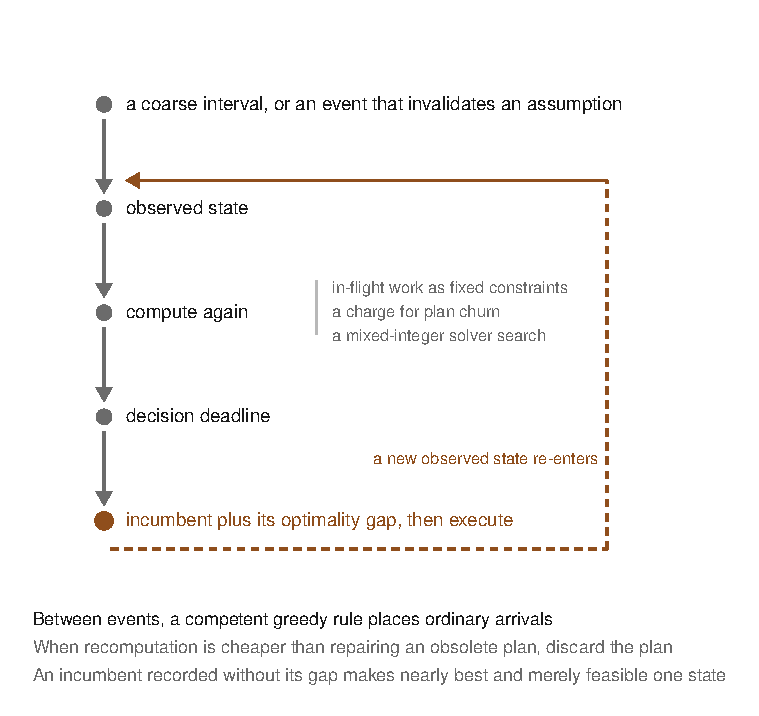
\includegraphics{figures/ch19-redecision-loop.pdf}
\caption{The re-decision loop recomputes from observed events under fixed work and churn costs, then executes a deadline capped incumbent while retaining its optimality gap.}
\end{figure}

Ordinary arrivals may use a cheap greedy rule between re-decision events. The system discards the existing plan only when the cost of recomputing is lower than the expected cost of executing or repairing an obsolete one.

\Needspace{5\baselineskip}

These terms identify the decisions that must be made before selecting an algorithm:

\begin{itemize}
\tightlist
\item
  What counts as sufficient performance?
\item
  How long may schedule computation run?
\item
  Which constraints are inviolable?
\item
  How is running work represented?
\item
  What reassignment cost counts as plan churn?
\item
  Which measure of remaining solution uncertainty must be retained?
\end{itemize}

The companion catalog contains algorithmic patterns. The narrower question here is whether these decisions lower accepted-result cost or improve flow on the fleet's own workload.

\hypertarget{when-should-the-scheduler-recompute-and-when-should-it-stop}{%
\section{When should the scheduler recompute, and when should it stop?}\label{when-should-the-scheduler-recompute-and-when-should-it-stop}}

An observatory scheduler can spend the night improving a plan that clouds have already invalidated, or compute another imperfect plan from the sky that remains observable. Bellm et al.~(\href{https://arxiv.org/abs/1905.02209}{2019}) describe the Zwicky Transient Facility taking the second approach in production since 2018. When changing conditions invalidate the schedule, it resolves the nightly integer program again rather than enumerating every weather scenario in advance.

Three directional observatory-scheduling sources support transferring this decision architecture to agent fleets. None provides a strong result for software fleets. The recommendation is therefore limited to choosing and measuring a re-decision policy. The appropriate cadence remains a local deployment decision.

The schedule should be treated as the current output of a control loop. At a coarse interval, or after an event invalidates an important assumption, the scheduler computes again from observed state. Between those points, a competent greedy rule can place ordinary arrivals without paying for a complete solve.

The system should abandon an obsolete plan when recomputation costs less than repairing or completing that plan. This comparison must include decision latency. An excellent schedule returned after the queue, capacity, or deadlines have changed is a schedule for a fleet that no longer exists.

\Needspace{5\baselineskip}

Current state includes more than queued work. Running tasks may:

\begin{itemize}
\tightlist
\item
  consume scarce model or execution capacity;
\item
  hold repository leases;
\item
  occupy reviewer slots;
\item
  have produced costly intermediate state; or
\item
  contain work another worker cannot reconstruct cheaply.
\end{itemize}

A re-solve should represent those commitments explicitly. Treating work in flight as fixed is a conservative default unless preemption has been separately justified.

The objective should also charge for \textbf{plan churn}: avoidable reassignment or resequencing that forces workers to discard useful preparation or partially completed work. Cadence, invalidation triggers, preemption, and churn penalties belong to the scheduling design rather than being added after the objective is chosen.

When the solve deadline arrives, execute the incumbent and retain its optimality gap. This follows from the mismatch between proof time and operational time. A solver may find a feasible plan quickly but take much longer to establish how close it is to the best plan. Meanwhile, new work arrives and the state used to construct the plan ages.

\Needspace{5\baselineskip}

The deadline prevents optimization itself from becoming another queue. The stored gap supports later questions:

\begin{itemize}
\tightlist
\item
  Did large gaps coincide with poorer flow?
\item
  Would more solve time have changed the executed assignments?
\item
  Did a tuned greedy policy perform just as well?
\item
  Did solve latency consume the predicted scheduling benefit?
\end{itemize}

Parazin et al.~(\href{https://arxiv.org/abs/2203.00013}{2022}) compared a mixed-integer scheduler for gravitational-wave follow-up with a tuned greedy heuristic. Neither won consistently. Under a 500-second cap, each performed better on different skymaps, and only 37 of 97 well-localized skymaps improved under the reported optimization comparison. Across 951 simulated events, a hybrid improved detection efficiency by roughly 3 to 11 percent. The authors also reported that reducing the cap to 100 seconds would have truncated only 64 additional schedules without a substantial efficiency loss.

\Needspace{5\baselineskip}

These are directional results from gravitational-wave follow-up rather than operating parameters for an agent fleet. They support evaluating:

\begin{itemize}
\tightlist
\item
  the solve deadline;
\item
  the retained gap;
\item
  the greedy baseline; and
\item
  a hybrid policy.
\end{itemize}

They argue against assuming that either the optimizer or the heuristic will win in advance.

Naghib et al.~(\href{https://arxiv.org/abs/1810.04815}{2019}) describe another observatory design in which a feature-based, memoryless policy chooses again from current state at every step. \emph{Memoryless} here does not mean that durable state is discarded. It means that the next scheduling action does not depend on preserving a brittle sequence of prior planned actions.

Interruptions are absorbed by observing the new state and making another decision. The evidence comes from a framework and simulation, so it supports a plausible architecture rather than a measured advantage for agent execution.

The fleet-wide and worker-local decisions should remain separate. A global allocator determines how scarce model tiers, reviewer capacity, or execution pools are divided among classes of work. A worker-local dispatcher determines which eligible item a particular worker takes next.

Combining both choices in one opaque score makes it difficult to determine whether a poor outcome arose from resource allocation or queue ordering. It can also allow local dispatch to undo a capacity decision the global layer just made.

The companion entry \texttt{formalize-work-as-constraints-and-solve-globally} proposes representing requests in one constraint language so an allocator can optimize across them. Its lineage reaches Hubble scheduling in 1990. The architecture is useful only when that representation captures the constraints operations actually enforce.

A nominally global solution built from missing deadlines, false independence assumptions, or omitted affinity constraints can be less coherent than separate local rules. The companion aside \texttt{audit-the-allocation-layer} therefore asks which policy actually controls execution, planning, and optimization. Its observatory analogy has no software-fleet measurement.

Probe costs belong in the same accounting. The thinly supported companion entry \texttt{probe-only-above-an-uncertainty-threshold} asks whether a dry run, canary, or classifier call reduces enough uncertainty to justify its latency and inference cost. Its theoretical constant comes from adversarial single-machine scheduling and does not transfer.

The local question is operational:

\begin{quote}
For which uncertain requests does a probe change the selected worker or schedule often enough to repay its cost?
\end{quote}

When logs cannot answer that question, probing remains another unmeasured allocation policy.

The evidence boundary should remain visible. The source survey does not cover much of the major USENIX and ACM cluster-scheduling literature. Agent runtime variance is also partly endogenous. Repeated tool failures, unstable environments, and unnecessary retries should be repaired at their source before the scheduler is asked to absorb them.

Nor does the cited evidence establish a general prohibition on preempting long-running agent sessions. Keeping running work fixed during a re-solve is a conservative representation of existing commitments rather than proof that preemption is always wrong.

Choose the cadence and solve deadline through a short pilot. Retain the incumbent, optimality gap, solve time, assignment decisions, and resulting execution trace at every re-decision. Compare the complete policy with a tuned greedy baseline.

The companion entry \texttt{pilot-to-pick-the-algorithm-then-commit-the-budget} states the same logic: spend a small amount distinguishing among methods, then commit the operating budget to the one that performs better.

\Needspace{5\baselineskip}

The design becomes auditable when the following are explicit:

\begin{itemize}
\tightlist
\item
  the re-decision trigger;
\item
  the solve deadline;
\item
  treatment of in-flight work;
\item
  the churn cost;
\item
  the simple baseline; and
\item
  the metrics used to compare them.
\end{itemize}

Its value remains an empirical question until the fleet's traces answer it.

\hypertarget{admission-backpressure-and-recovery-capacity}{%
\section{Admission, backpressure, and recovery capacity}\label{admission-backpressure-and-recovery-capacity}}

In the eleven-week replay described later in this chapter, the scheduling effect concentrated entirely in one contended pool, where eligible work regularly exceeded available capacity; the uncontended pool showed almost no difference across policies. That retained observation locates where overload policy matters: not everywhere, but at the resources where demand exceeds capacity, and most acutely when capacity has just fallen. A queue records demand; it does not create capacity. Retry policy can increase demand precisely when capacity has fallen. A reliable factory therefore needs overload policy above individual queues, distinct from the re-decision and routing questions elsewhere in this chapter: those decide which work runs where, and overload policy decides how much work is allowed to exist inside the system at all.

The failure mode this section guards against is mechanical. A dependency slows, tasks time out, retries multiply the request rate against the slowed dependency, queues grow, work waits long enough that its callers retry the whole task, and the fleet spends its capacity on demand that its own policies manufactured. Nothing in that sequence requires a model to misbehave. The Google SRE chapters on \href{https://sre.google/sre-book/addressing-cascading-failures/}{cascading failures} and \href{https://sre.google/sre-book/handling-overload/}{handling overload} describe this pattern across production services; I cite them as practitioner guidance rather than controlled evidence, and none of their capacity or threshold figures transfer to an agent fleet. The figure below shows the amplification loop and the policies that bound it. Overload policy has three responsibilities: bound total admitted demand, prevent one ownership or workload domain from consuming the fleet, and release retry and recovery traffic at a controlled rate.

\begin{figure}[htbp]
\centering
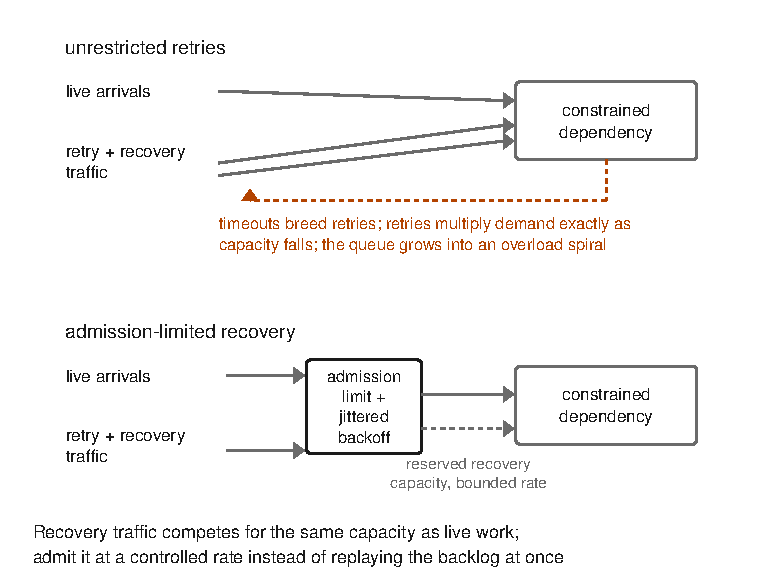
\includegraphics[width=1\textwidth,height=\textheight,keepaspectratio]{figures/ch19-recovery-backpressure.pdf}
\caption{Live arrivals and retry-driven recovery traffic compete for the same constrained dependency; unrestricted retries amplify load exactly when capacity has fallen, while admission limits, jitter, and reserved recovery capacity bound the interference.}
\end{figure}

\textbf{Bounding admitted demand.} The first policy decision is whether new work enters the system at all. Verma et al.~(\href{https://research.google/pubs/large-scale-cluster-management-at-google-with-borg/}{2015}) describe Borg holding submitted jobs in a pending state until admission, packing admitted work against declared resource requirements, isolating tenants, and treating overcommitment as an explicit cluster policy rather than an accident of scheduling. The transfer is directional: an agent fleet benefits from the same separation between accepting work and running it, and from making overcommitment a decision with an owner. Borg's packing algorithms, machine-share targets, and utilization figures do not transfer as parameters.

Admission requires bounded queue growth. An unbounded queue converts overload into unbounded latency, and by contract I9 admissible work cannot starve invisibly. A bounded queue forces the honest alternatives into view: reject explicitly, shed load by declared class, or wait with a visible position and age. Explicit rejection at admission is cheaper than the same rejection discovered hours later as a timeout, because the caller learns immediately and the system spends nothing executing work it will abandon. When a downstream stage saturates, the signal must propagate upstream as backpressure rather than accumulate in an intermediate queue; when slowing is not enough, the system sheds load by explicit policy, rejecting the lowest declared class first and telling the caller. Silent degradation, where work is accepted and then quietly never runs, violates I9 directly.

\textbf{Isolating demand domains.} Aggregate capacity limits are not enough, because a single hot tenant or repository can fill a shared queue and starve unrelated work while the aggregate limit is still respected. Partitioning queues by tenant, repository, or work class bounds the damage one demand source can do to another. Mace et al.~(\href{https://www.usenix.org/conference/nsdi15/technical-sessions/presentation/mace}{2015}) built Retro around per-tenant resource monitoring and central control points that throttle at the granularity of the tenant, and they observed that maintenance traffic itself can become the overload source. Both observations transfer directionally. In an agent fleet, the analogue of maintenance traffic is recovery, reconciliation, and retry work, and it competes for the same models, runners, and reviewers as live work.

\textbf{Concurrency limits by constrained resource.} Concurrency limits belong on the resource that is actually constrained, not on an arbitrary global worker count. Model-tier tokens per minute, repository leases, reviewer attention, and external API rate limits are separate constraints with separate saturation points. A single fleet-wide concurrency number either wastes the uncontended resources or oversubscribes the contended one. The contended-pool observation from my replay applies here in reverse: limits matter where eligible work exceeds capacity, and a limit on an uncontended resource is dead configuration.

\textbf{Retry budgets, backoff, and jitter.} Retries are the mechanism by which demand rises as capacity falls, so they need a budget, not just a count. A per-attempt retry cap still permits a retry storm when many attempts fail together; a budget bounds the fraction of total traffic that retries may consume. Individual retries should back off exponentially, and backoff must carry jitter, because deterministic backoff synchronizes the failed population into retry waves that arrive together and re-saturate the recovering dependency. The AWS Builders' Library articles on \href{https://aws.amazon.com/builders-library/timeouts-retries-and-backoff-with-jitter/}{timeouts, retries, and backoff with jitter} and on \href{https://aws.amazon.com/builders-library/making-retries-safe-with-idempotent-APIs/}{making retries safe with idempotent APIs} state both mechanisms clearly; they are practitioner guidance, and their specific multipliers and cap values are their systems' parameters, not this book's. The idempotency requirement is not optional decoration here. A retry is a new attempt at the same logical work (contract I4), and a retried external effect is safe only under the effect-identity contracts of I5. A retry policy layered over non-idempotent effects converts overload into duplicated external commits.

\textbf{Recovery capacity.} Recovery and reconciliation need their own capacity policy, so that backlog cannot consume every worker needed to recover it. After a worker loss or a dependency outage, the system holds a backlog of interrupted attempts, orphaned leases, and unreconciled external effects. Recovering those requires the same constrained resources as live work. If the backlog is admitted at full priority into an undifferentiated queue, recovery work and live work starve each other, and the reconciliation that would shrink the backlog never gets scheduled. Contract I10 requires that recovery preserve the same obligations as normal execution and be tested as production code; that includes its capacity allocation. A recovery path that only works when the fleet is idle has not been tested under the one condition where it runs. Pilot-execution work by Li, Cai, and Lou (\href{https://www.usenix.org/conference/nsdi26/presentation/li-zhenyu}{2026}) adds the sharper directional warning that recovery actions themselves cause severe failures, which is a second reason to bound the rate at which recovery traffic is released rather than replaying the entire backlog at once. No universal fraction of capacity is prescribed here for recovery. That is a measured deployment decision, and the experiment below is how to measure it.

The global-allocation versus worker-local-dispatch separation defended earlier in this chapter has a precedent in this literature. Schwarzkopf et al.~(\href{https://research.google/pubs/omega-flexible-scalable-schedulers-for-large-compute-clusters/}{2013}) built Omega as parallel schedulers operating over shared cluster state with optimistic concurrency control, precisely because a single monolithic scheduler conflated policies with different cadences and stakes. Hindman et al.~(\href{https://www.usenix.org/conference/nsdi11/mesos-platform-fine-grained-resource-sharing-data-center}{2011}) reached a related two-level split in Mesos, with a central allocator offering resources and frameworks deciding what to run on them. Both are directional support for keeping capacity allocation and dispatch as separately auditable layers; neither system's conflict rates, offer semantics, or scale figures describe an agent fleet.

\Needspace{5\baselineskip}

The replay protocol later in this chapter tests dispatch policy under normal arrivals. Overload policy needs its own experiment, because its interesting behavior only appears when capacity falls or backlog is released. I add a recovery-capacity experiment to the protocol:

\begin{enumerate}
\def\labelenumi{\arabic{enumi}.}
\tightlist
\item
  Establish the normal arrival rate and the capacity of each constrained resource from the ledger.
\item
  Inject a worker loss or a dependency failure of recorded duration.
\item
  Release a controlled backlog and retry population against the recovering system.
\item
  Compare unrestricted recovery traffic with a bounded-recovery policy that reserves declared capacity for live work and admits recovery work at a controlled rate.
\item
  Measure, by declared class: live-work tail latency, recovery completion time, queue depth, retry count, request rate against the recovering dependency, starvation against the existing guard, useful throughput, and duplicate external effects.
\end{enumerate}

The comparison should show where each policy fails, not which one wins in general. Unrestricted recovery typically minimizes recovery completion time while damaging live-work tails and re-saturating the dependency; an over-tight bound protects live work while the backlog ages past usefulness. The right division is a property of the fleet's own workload, which is why this section gives an experiment rather than a universal recovery-capacity fraction.

\hypertarget{which-worker-is-cheapest-and-sufficient}{%
\section{Which worker is cheapest and sufficient?}\label{which-worker-is-cheapest-and-sufficient}}

Cheapest-sufficient routing has support from three directional literature items and one recent benchmark-bound controlled result. Cayci, Eryilmaz, and Srikant (\href{https://arxiv.org/abs/2003.00365}{2020}) developed budget-constrained online learning under broad cost and reward distributions. Somerstep et al.~(\href{https://arxiv.org/abs/2502.03261}{2025}) analyzed a calibrated static router. Li (\href{https://arxiv.org/abs/2502.02743}{2025}) reported preference-conditioned dynamic routing in a single-author preprint.

None evaluates a production software-agent fleet. This section therefore defines the routing decision and the measurements required to test it. It does not establish that a learned router will lower the cost of a particular fleet.

My fleet orchestrator illustrates the starting point. Each execution pool has a model assigned through a static configuration string. There is no request-level performance estimate, cost model, deadline, or lookahead.

The static table is predictable and legible. It also supplies the fallback when a selective router lacks evidence. Its limitation is that dispatch cannot respond to variation in request difficulty.

\Needspace{5\baselineskip}

A cheapest-sufficient router replaces the static assignment with two estimates for every candidate worker on the current request:

\begin{itemize}
\tightlist
\item
  expected task performance; and
\item
  expected total cost.
\end{itemize}

It then selects the least expensive worker predicted to satisfy the declared requirement.

Bhola, Krishnan, and NS (\href{https://arxiv.org/abs/2608.04804}{2026}) evaluated a scout-and-route configuration on 266 Python tasks from SWE-bench Pro. It solved 159 tasks, compared with 158 for the best single model, at about one fifth of the reported total cost per solve. A no-router ablation that always selected the cheapest fixer but retained the verified handoff tied the routed system, locating the measured gain in the handoff rather than the routing decision. The result strongly supports that benchmark-specific configuration and its null routing ablation; generalized cheapest-sufficient routing remains directional.

Somerstep et al.~analyze this plug-in structure in CARROT and argue that its direct routing overhead is negligible because selection requires evaluating the two predictors for each available model. The useful behavior still depends on calibration: predicted performance must correspond to observed performance on the deployment distribution.

A mathematically correct selector cannot compensate for a predictor that assigns unjustified confidence to unfamiliar work.

\Needspace{5\baselineskip}

The sufficiency requirement must be operational rather than rhetorical. ``Good enough'' might mean:

\begin{itemize}
\tightlist
\item
  passing an executable verifier;
\item
  remaining below a defect-probability threshold;
\item
  satisfying a calibrated review rubric;
\item
  meeting a deadline;
\item
  preserving a reliability requirement; or
\item
  satisfying a caller-selected cost-quality tradeoff.
\end{itemize}

Each defines a different routing problem.

The roughly 15-fold token premium reported for some fan-out configurations in Chapter 18 makes this choice economically consequential. Token count is still not the final objective. A cheap model that triggers repeated repair, verification, and review can cost more per accepted result than a stronger model would have cost initially.

When sufficient outcome data accumulates, the router can update through a budget-constrained bandit, such as Thompson sampling, with the algorithmic details left to the companion catalog. Cayci, Eryilmaz, and Srikant establish an asymptotic regret guarantee under moment conditions that permit heavy-tailed, correlated, and even negative cost-reward pairs.

Those properties resemble agent dispatch more closely than a setting with bounded independent rewards. The guarantee does not tell an operator whether the reward represents useful software work, and it provides limited guidance during the early period when production exploration is most costly.

Online updating addresses a real limitation of static routing. Models and workloads change. A model revision can change which tier is sufficient. A new repository or task family can move requests outside the router's calibration population.

Li conditions routing on a user-selected performance-cost preference, allowing one learned policy to represent several tradeoffs at inference time. The evidence is benchmark-based and comes from a single-author preprint. It supports testing preference conditioning. Calibration under delayed software outcomes remains unmeasured.

\Needspace{5\baselineskip}

The reward definition is the controlling measurement choice. Software signals arrive at different times and answer different questions:

\begin{itemize}
\tightlist
\item
  tests may be immediate but incomplete;
\item
  review may identify defects later;
\item
  rework or rollback may occur after acceptance;
\item
  user rejection may arrive after the router has recorded success; and
\item
  review effort may erase the apparent savings of the selected model.
\end{itemize}

Combining those signals into one reward is a construct-validity decision outside the routing mathematics. The reward definition should be versioned so that policies trained under different meanings of success are not silently compared.

\Needspace{5\baselineskip}

A learned policy should remain advisory until its recommendations correlate with an outcome measured outside the router and relevant to accepted work. In advisory mode, record:

\begin{itemize}
\tightlist
\item
  the requested route;
\item
  the route actually taken;
\item
  predicted performance;
\item
  predicted cost;
\item
  uncertainty;
\item
  the routing reason; and
\item
  the eventual outcome.
\end{itemize}

The thinly supported companion entry \texttt{log-scheduling-decisions-for-selection-effect-modeling} adds an important field: why the request received that route. Without the selection reason, later analysis cannot distinguish model quality from the policy that sent different work to each model.

When observations are sparse, fall back to the static cost-performance table. That floor is the current configuration and can be measured directly. The learned router should take control only where its errors can be estimated with adequate density.

Rare task families, new models, and new reward definitions should remain on the static floor until the router exposes enough evidence and uncertainty to justify a different choice.

\Needspace{5\baselineskip}

Calibration can fail before deployment. Benchmark-derived routing data may encode:

\begin{itemize}
\tightlist
\item
  regular prompt formats;
\item
  benchmark-specific scoring;
\item
  an unrealistically fixed model menu;
\item
  task distributions unlike production; or
\item
  missing repair and review costs.
\end{itemize}

CARROT assumes a static model pool. Production pools change as prices move, versions are retired, rate limits vary, and tool compatibility excludes some models. Each change requires recalibration or creates a region in which the router is extrapolating.

Online exploration creates another cost. A learning policy must sometimes choose an uncertain worker to gather information, and the routed request is real production work. A budget constraint reveals the cost but does not decide who may bear it.

\Needspace{5\baselineskip}

Deployment therefore needs:

\begin{itemize}
\tightlist
\item
  an exploration budget;
\item
  exclusions for high-consequence work;
\item
  a stop condition tied to routing error;
\item
  a static fallback; and
\item
  a record of which production requests were used for learning.
\end{itemize}

An asymptotic guarantee does not excuse poor performance during the learning period.

The companion pattern \texttt{cost-cascade-routing} provides another response to uncertainty. Begin with a cheaper route and escalate when calibrated confidence is insufficient. Chang (\href{https://arxiv.org/abs/2604.12262}{2026}) reports that confidence-gated cascades often outperformed always-on strong-model fan-out in both cost and quality.

That result supports the catalog pointer rather than a universal deployment rule. A cascade changes latency and couples its stages through the escalation signal. It must be evaluated as one complete route, with cost measured across every call.

A routing decision record should include:

\Needspace*{15\baselineskip}
\begin{verbatim}
sufficiency_requirement:
reward_version:
calibration_population:
model_pool_version:
predicted_performance:
predicted_cost:
uncertainty:
routing_reason:
exploration_budget:
static_fallback:
eventual_outcome:
accepted_result_cost:
\end{verbatim}

Evaluation should report cost per accepted result and failure rates by request class, not only average token use.

Cheapest-sufficient routing is useful because it makes the economic policy explicit: what is being predicted, what requirement must be met, and which tradeoff is being selected. It cannot repair an unrepresentative calibration set, a reward that measures the wrong outcome, or a task whose true cost appears only after repair and review.

\hypertarget{does-the-policy-survive-a-fixed-arrival-replay}{%
\section{Does the policy survive a fixed-arrival replay?}\label{does-the-policy-survive-a-fixed-arrival-replay}}

In one replay of my agent fleet, the interesting scheduling idea lost to a one-word configuration change. Across eleven weeks of recorded traffic, a four-feature weighted index performed within 0.1 percent of plain priority banding.

That result has narrative value only and is not primary evidence for this practice. The strong support comes from SWAY, the controlled software-engineering study by Chen et al.~(\href{https://arxiv.org/abs/1608.07617}{2016}), which shows why a proposed search method should have to beat a cheap baseline. Decima, from Mao et al.~(\href{https://arxiv.org/abs/1810.01963}{2018}), and the telescope-network work of Lampoudi, Saunders, and Eastman (\href{https://arxiv.org/abs/1503.07170}{2015}) provide directional support for learned scheduling and validation against known optima.

Fixed-arrival replay itself remains a reasoned transfer rather than a controlled result from an agent fleet.

An \textbf{arrival trace} is a time-ordered record of work entering the system, including the information available when each item arrived. A \textbf{dispatch policy} decides which eligible item receives a resource next. \textbf{First-come scheduling} orders eligible work by arrival time, subject to constraints that make an item impossible to run.

A \textbf{replay harness} re-executes the recorded arrivals under a candidate dispatch policy without changing production state. It differs from the single-run replay used for debugging in Chapter 10. That replay reconstructs one execution. This harness holds an entire workload sequence fixed while replacing the policy that allocates it.

\Needspace{5\baselineskip}

The trace needs, at minimum:

\begin{itemize}
\tightlist
\item
  arrival time;
\item
  priority;
\item
  resource eligibility;
\item
  claims and releases;
\item
  observed duration;
\item
  completion or failure outcome;
\item
  review verdict; and
\item
  work already running at each decision.
\end{itemize}

It also needs any constraint that affected feasibility. If the historical record omits capacity, cancellation, model compatibility, repository leases, or work already in flight, the replay may create choices the live scheduler never had.

Missing decision context is not neutral noise. It changes the feasible schedule.

Holding arrivals fixed creates a paired comparison. Every policy encounters the same demand in the same order. Differences in simulated flow can therefore be attributed to the policy and its interaction with the reconstructed state rather than to one arm receiving a busier week.

The replay is not causal in every respect. It does remove one large source of variation that often overwhelms scheduler comparisons.

\Needspace{5\baselineskip}

The first run should validate the harness rather than compare policies. Construct small cases whose best schedule is known, including:

\begin{itemize}
\tightlist
\item
  simultaneous arrivals;
\item
  a resource becoming unavailable;
\item
  a priority inversion;
\item
  incompatible execution pools;
\item
  a cancellation while work is queued; and
\item
  work already in flight when a new item arrives.
\end{itemize}

Confirm that the replay clock, eligibility logic, claim duration, completion events, and resource accounting reproduce the expected schedule.

Lampoudi, Saunders, and Eastman (2015) derived an integer-program formulation for the Las Cumbres Observatory network and reported computational validation at realistic problem sizes. The transferable practice is to test the scheduling kernel on instances with known answers before trusting its output on a historical trace.

\Needspace{5\baselineskip}

The second run establishes cheap baselines. Compare the proposed policy with:

\begin{itemize}
\tightlist
\item
  first-come scheduling;
\item
  a simple priority sort;
\item
  a tuned greedy rule; and
\item
  random oversampling.
\end{itemize}

Random oversampling generates several inexpensive randomized schedules and retains the best under the declared objective. Chen et al.~(2016) developed SWAY by sampling a large candidate population down to better solutions rather than evolving many generations. Across several software-engineering models, it was competitive with state-of-the-art evolutionary algorithms at substantially lower computational cost. The authors proposed it explicitly as a baseline for search-based software engineering.

The controlled result supports the discipline: an elaborate optimizer that cannot beat a cheap alternative has not earned adoption.

\Needspace{5\baselineskip}

The objective must be fixed before inspecting the policy results. Possible objectives include:

\begin{itemize}
\tightlist
\item
  mean completion time;
\item
  priority-weighted flow time;
\item
  deadline misses;
\item
  accepted-result cost;
\item
  reviewer delay; and
\item
  time spent blocked on a constrained resource.
\end{itemize}

These measures describe different failures. A lower fleet-wide mean can coexist with severe delay for one priority or request class.

\textbf{Starvation} is persistent denial or extreme delay to a class because other eligible work repeatedly moves ahead of it. Report outcomes by class and define a starvation guard before running the comparison. An aggregate gain is not acceptable when one class pays for it through unbounded delay.

The opening replay also moved P1 tail latency from 20.4 hours to 18.8 hours without triggering the starvation guard. Those figures explain what the protocol prevented me from building; they are not an expected gain for another fleet.

Capacity distribution explained more than the aggregate result. The visible improvement concentrated in one \textbf{contended pool}, where eligible work regularly exceeded available capacity. An \textbf{uncontended pool}, where capacity usually met demand, showed almost no difference across policies.

That is the expected shape of a genuine scheduling effect. When work rarely waits for a resource, queue order has little opportunity to change the outcome. A policy claiming large gains in an uncontended pool deserves scrutiny.

Decima provides a useful but bounded comparison. Mao et al.~(2018) trained a cluster scheduler under continuous stochastic arrivals and evaluated it on a 25-node Spark cluster. They reported at least a 21 percent improvement in average job-completion time over hand-tuned heuristics, with gains reaching approximately twofold under high load.

Those measurements support learned scheduling in that cluster environment. They do not evaluate fixed-arrival replay and do not establish an expected effect for agent work. The transferable experimental rule is narrower: preserve the arrival process when comparing policies and look for gains where resources are actually contested.

\Needspace{5\baselineskip}

Historical replay also preserves historical selection. Work absent from the ledger remains absent, including:

\begin{itemize}
\tightlist
\item
  requests users never submitted because the old system was slow;
\item
  tasks operators diverted manually;
\item
  work rejected before entering the queue; and
\item
  difficult requests routed to another worker group.
\end{itemize}

A route may therefore contain an artificially easy trace because the incumbent policy sent hard work elsewhere. The companion entry \texttt{log-scheduling-decisions-for-selection-effect-modeling} adds the reason each item entered a route, allowing later analysis to model selection. It cannot reconstruct demand that was never observed.

A live policy can also change future arrivals. Faster completion may create more demand. Priority treatment may change how users label requests. Model routing can change reviewer behavior and the kinds of tasks people submit.

\Needspace{5\baselineskip}

Historical replay cannot capture all such feedback. Use a \textbf{temporal holdout}, a later period excluded while policies are developed, to test whether the replay result survives workload drift. Then stage deployment through:

\begin{enumerate}
\def\labelenumi{\arabic{enumi}.}
\tightlist
\item
  shadow evaluation;
\item
  one-project or one-pool canary;
\item
  bounded live authority; and
\item
  fleet-wide rollout.
\end{enumerate}

Each stage should retain an external outcome measure and the starvation guard.

\Needspace{5\baselineskip}

A compact replay protocol is:

\begin{enumerate}
\def\labelenumi{\arabic{enumi}.}
\tightlist
\item
  Export an immutable arrival trace containing decisions, resources, claims, durations, outcomes, and review verdicts.
\item
  Build a discrete replay clock and validate the scheduler on constructed cases with known answers.
\item
  Record the objective, class-specific starvation guard, acceptance threshold, and cost accounting before comparing policies.
\item
  Replay first-come scheduling, simple priority, a tuned cheap baseline, random oversampling, and each candidate over the identical trace.
\item
  Report aggregate and per-class outcomes, decision cost, contention location, and optimality information where available.
\item
  Repeat the comparison on a temporal holdout.
\item
  Require shadow and canary evidence before expanding live allocation authority.
\item
  Run the recovery-capacity experiment from the admission and backpressure section: establish normal arrival rate and capacity, inject a worker loss or dependency failure, release a controlled backlog and retry population, and compare unrestricted recovery traffic with a bounded-recovery policy on live-work tail latency, recovery completion time, per-class queue depth, retry count, dependency request rate, starvation, useful throughput, and duplicate external effects.
\end{enumerate}

\Needspace{5\baselineskip}

This protocol is stricter than asking whether the queue feels better. It asks:

\begin{itemize}
\tightlist
\item
  whether the candidate changes a declared outcome on identical work;
\item
  whether a trivial policy captures the same gain;
\item
  whether one class pays for the improvement;
\item
  whether the effect occurs where capacity is constrained; and
\item
  whether it survives later traffic.
\end{itemize}

If the ledger already records the required state, the harness can be built without changing production scheduling. If it does not, the immediate scheduling task is instrumentation.

The earlier decisions in this chapter then become hypotheses rather than received settings. Replay several re-decision cadences and solve limits while preserving in-flight work. Measure flow, churn, solve latency, and the optimality gap retained at each limit.

Replay cheapest-sufficient routes from logged estimates when counterfactual outcomes are available. Otherwise run them in shadow. Measure accepted-result cost and calibration error by request class.

Build the trace, hold arrivals fixed, make the cheap policy compete, and let the fleet produce the evidence its allocation policy requires.

\hypertarget{what-must-be-recorded-before-optimization}{%
\section{What must be recorded before optimization?}\label{what-must-be-recorded-before-optimization}}

When the ledger does not preserve decision state, add fields in dependency order.

\begin{longtable}[]{@{}
  >{\raggedright\arraybackslash}p{(\columnwidth - 2\tabcolsep) * \real{0.5000}}
  >{\raggedright\arraybackslash}p{(\columnwidth - 2\tabcolsep) * \real{0.5000}}@{}}
\caption{Allocation-ledger fields in the order they become interpretable.}\tabularnewline
\toprule\noalign{}
\begin{minipage}[b]{\linewidth}\raggedright
Stage
\end{minipage} & \begin{minipage}[b]{\linewidth}\raggedright
Fields
\end{minipage} \\
\midrule\noalign{}
\endfirsthead
\toprule\noalign{}
\begin{minipage}[b]{\linewidth}\raggedright
Stage
\end{minipage} & \begin{minipage}[b]{\linewidth}\raggedright
Fields
\end{minipage} \\
\midrule\noalign{}
\endhead
\bottomrule\noalign{}
\endlastfoot
Observed events & Arrival time, priority, claim and release events, observed duration, completion or failure outcome, and review verdict. \\
Decision state & Available capacity, eligible execution pools, work already running, leases or locks, deadlines, model or tool compatibility, reviewer availability, and constraints that excluded an otherwise eligible item. \\
Policy estimates & Predicted cost, predicted task performance, routing uncertainty, expected duration, solver objective value, and optimality gap. \\
Code-estate state & Campaign identity, repository, base revision, host or workspace, affected entities, artifact version, code index version, conflict evidence, and publication state. \\
\end{longtable}

The observed fields reconstruct demand, occupancy, and accepted work. They also expose missing or contradictory histories before policy-specific estimates complicate the schema.

Record the route selected and the reason for that route in the same decision event. State and reason need a shared decision identity and timestamp. Without them, later analysis cannot determine which alternatives were feasible or distinguish worker performance from the policy that selected the work.

The code-estate fields carry the same versioned view of the code that Chapter 18's node record gives the task graph into the allocation ledger, so that a scheduling decision can later be checked against the repository state and conflict evidence it acted on; full cross-repository campaign semantics stay in the companion repository, because the current evidence does not support a developed practice claiming one campaign protocol is generally superior.

Estimates belong last because they are outputs of a policy rather than observations of what happened. Store the policy, model, feature, and reward versions that produced them. Recalibration should create a new estimate record rather than rewrite the historical one.

The first operating comparison can remain descriptive. Ask whether high-throughput intervals under the incumbent policy also have a higher accepted-result cost than lower-throughput intervals. Report both measures by request class and constrained resource.

That comparison cannot establish the counterfactual effect of a new router, the correct re-decision cadence or solver limit, an exploration guarantee, the effect of demand absent from the ledger, or the causal effect of throughput on accepted-result cost.

Those questions still require replay, shadow execution, or controlled rollout on the fleet's workload. None of the cited studies reports results from a software-agent fleet.

My replay supplies no default cadence, threshold, or cost ratio. Do not import an observatory schedule, a bandit guarantee, or my 15 percent promotion rule.

The useful outcome is an allocation record that reconstructs what arrived, what was eligible, which resources and alternatives existed, which policy selected the route and why, what the work cost, what outcome survived review, and which later events changed the interpretation of the result.

Until the ledger can answer those questions, choosing a more sophisticated policy is premature.

The repository artifact \href{https://github.com/sjarmak/engineering-reliable-coding-agents/blob/main/protocols/allocation-policy-replay.md}{\texttt{protocols/allocation-policy-replay.md}} defines the replay comparison, promotion rule, and retained decision record.

\section*{Sources and evidence}

\textbf{Re-decide cheaply and ship the incumbent}

\begin{itemize}
\tightlist
\item
  Directional evidence: Bellm, E. C., et al.~(2019), ``The Zwicky Transient Facility: Surveys and Scheduler,'' PASP 131, 068003, arXiv:1905.02209.
\item
  Directional evidence: Naghib, E., et al.~(2018/2019), ``A Framework for Telescope Schedulers: With Applications to the Large Synoptic Survey Telescope,'' AJ 157, 151 (2019), arXiv:1810.04815 (2018). Framework and simulation evidence.
\item
  Directional evidence: Parazin, B., et al.~(2022), ``Foraging with MUSHROOMS: A Mixed-integer Linear Programming Scheduler for Multimessenger Target of Opportunity Searches with the Zwicky Transient Facility,'' ApJ 935, 87, arXiv:2203.00013.
\item
  Strong evidence for production workload characterization, directional for capacity-policy transfer: Liu, B., et al.~(2026), ``Agentic Coding in the Wild: Characterizing GitHub Copilot Traces at Production Scale,'' arXiv:2608.00101.
\item
  No strong result and no software-fleet measurement support this entry; all three items are observatory scheduling, and the cadence, cap, and churn charge remain deployment decisions.
\item
  Corroboration (narrative only): the author's transfer notes on observatory scheduling restate the same ZTF and MUSHROOMS results already carried above as literature evidence.
\end{itemize}

\textbf{Admission, backpressure, and recovery capacity}

\begin{itemize}
\tightlist
\item
  Directional evidence: Verma, A., et al.~(2015), ``Large-scale cluster management at Google with Borg,'' EuroSys. Admission control, packing, isolation, and overcommitment as explicit cluster policy; mechanisms transfer, parameters do not.
\item
  Directional evidence: Schwarzkopf, M., et al.~(2013), ``Omega: flexible, scalable schedulers for large compute clusters,'' EuroSys. Parallel schedulers over shared state with optimistic concurrency; supports separating global allocation from worker-local dispatch.
\item
  Directional evidence: Mace, J., et al.~(2015), ``Retro: Targeted Resource Management in Multi-tenant Distributed Systems,'' NSDI. Per-tenant resource monitoring and central control points; maintenance and recovery traffic can itself become the overload source.
\item
  Directional evidence: Hindman, B., et al.~(2011), ``Mesos: A Platform for Fine-Grained Resource Sharing in the Data Center,'' NSDI. Two-level allocation between a central allocator and per-framework dispatch.
\item
  Directional evidence: Li, Z., Cai, Q., \& Lou, C. (2026), ``Pilot Execution,'' NSDI. Recovery actions themselves cause severe failures; supports bounding the release rate of recovery traffic.
\item
  Practitioner guidance: AWS Builders' Library, ``Timeouts, retries, and backoff with jitter'' and ``Making retries safe with idempotent APIs.'' Mechanism descriptions from production practice, not controlled experiments; their constants are their systems' parameters.
\item
  Practitioner guidance: Google SRE, ``Addressing Cascading Failures'' and ``Handling Overload.'' Same status.
\item
  No source in this group evaluates a software-agent fleet, and no recovery-capacity fraction is prescribed; the recovery-capacity experiment in the replay protocol is how a fleet measures its own division.
\end{itemize}

\textbf{Route each request to the cheapest sufficient model}

\begin{itemize}
\tightlist
\item
  Directional evidence: Cayci, S., Eryilmaz, A., \& Srikant, R. (2020), ``Budget-Constrained Bandits over General Cost and Reward Distributions,'' arXiv:2003.00365. Asymptotic guarantee under stated moment conditions.
\item
  Directional evidence: Somerstep, S., et al.~(2025), ``CARROT: A Cost Aware Rate Optimal Router,'' arXiv:2502.03261. Static model pool assumed.
\item
  Directional evidence: Li, Y. (2025), ``LLM Bandit: Cost-Efficient LLM Generation via Preference-Conditioned Dynamic Routing,'' arXiv:2502.02743. Single-author preprint, benchmark evidence.
\item
  Strong evidence for one benchmark-bound scout-and-fixer configuration and its no-router ablation: Bhola, I., Krishnan, A., and NS, M. (2026), ``Scrouting: Cost-Aware Routing of Coding Agents by Scouting the Repository First,'' arXiv:2608.04804. The handoff, rather than the router, carried the measured result.
\item
  The three routing-theory items remain directional, and no source evaluates a production software-agent fleet; generalized cheapest-sufficient routing therefore remains a decision to test rather than an established cost reduction.
\item
  Directional evidence for this developed practice: CascadeDebate (Chang 2026), arXiv:2604.12262. Its confidence-gated cascade comparison strongly supports the narrower companion-catalog claim in the tested setting; transfer to production software-agent routing remains directional.
\item
  Corroboration (narrative only): the author's transfer notes restate the budgeted-bandit formulation already carried above.
\end{itemize}

\textbf{Replay fixed arrival traces before changing policy}

\begin{itemize}
\tightlist
\item
  Strong evidence for the cheap-baseline comparison only: SWAY, Chen, J., et al.~(2016), ``Sampling as a Baseline Optimizer for Search-Based Software Engineering,'' arXiv:1608.07617. The study supports requiring a candidate optimizer to beat a cheap baseline; fixed-arrival replay is a transfer beyond its experiment.
\item
  Directional evidence: Decima, Mao, H., et al.~(2018), ``Learning Scheduling Algorithms for Data Processing Clusters,'' arXiv:1810.01963. Measures learned scheduling under stochastic arrivals, not fixed-arrival replay; the replay transfer is the synthesis's.
\item
  Directional evidence: Lampoudi, S., Saunders, E., \& Eastman, J. (2015), ``An Integer Linear Programming Solution to the Telescope Network Scheduling Problem,'' arXiv:1503.07170. Supports validating a scheduling kernel on instances with known optima.
\item
  Fixed-arrival replay itself is a reasoned transfer, not a directly controlled fleet result, and per-class starvation must be checked separately because a policy can improve the mean by starving one class.
\item
  Corroboration (illustration only): the author's eleven-week replay of 1,286 work items across 22 execution pools, and the author's shadow, canary, then fleet rollout design. These cases do not count as independent external evidence.
\end{itemize}
